\section{Bonus: Combined Regularization Strategy}

\subsection{Implementation}

To maximize performance while avoiding overfitting, I implemented \textbf{both strategies together}: dropout + early stopping in a single model.

\textbf{Code modifications:}
\begin{lstlisting}[language=Python]
# MLPWithDropout class with dropout_rate=0.3
combined_mlp = MLPWithDropout(dropout_rate=0.3)
optimizer = optim.Adam(combined_mlp.parameters(), lr=0.001)

# Train with early stopping patience=5
combined_history = train_model(
    combined_mlp, train_loader, val_loader, 
    criterion, optimizer,
    num_epochs=50, early_stopping_patience=5
)
\end{lstlisting}

\subsection{Results}

\begin{figure}[h]
    \centering
    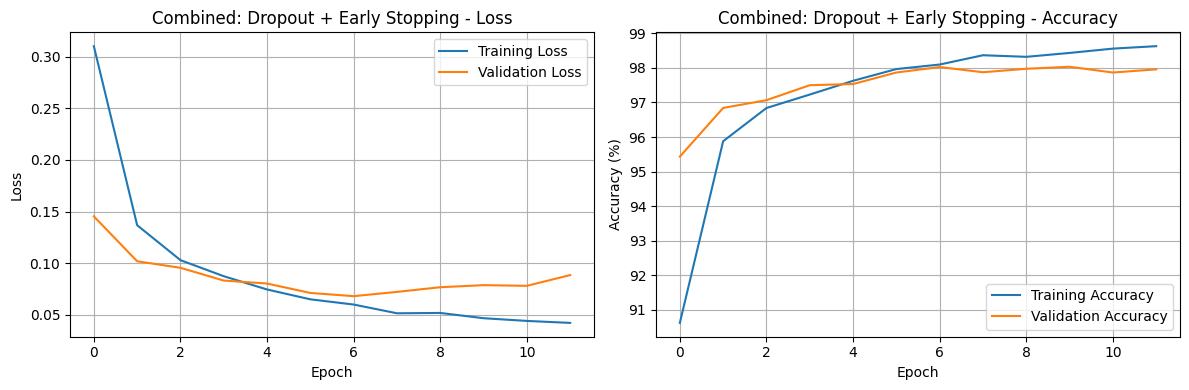
\includegraphics[width=0.7\linewidth]{section6/combined.png}
    \caption{Combined strategy: Dropout + Early Stopping working together}
    \label{fig:combined}
\end{figure}

\begin{table}[h]
\centering
\begin{tabular}{|l|c|c|c|}
\hline
\textbf{Strategy} & \textbf{Val Acc} & \textbf{Epochs} & \textbf{Train-Val Gap} \\ \hline
Baseline & 97.87\% & 50 & 1.91\% \\ \hline
Dropout only & 98.09\% & 50 & 1.32\% \\ \hline
Early Stop only & 97.72\% & 10 & 1.80\% \\ \hline
\textbf{Combined} & \textbf{97.96\%} & \textbf{12} & \textbf{0.67\%} \\ \hline
\end{tabular}
\caption{Performance comparison of regularization strategies}
\label{tab:combined-results}
\end{table}

\subsection{Analysis}

The combined approach achieves the \textbf{best generalization performance}:
\begin{itemize}
    \item \textbf{Minimal overfitting}: Train-val gap of only 0.67\%—the lowest among all methods, indicating excellent generalization
    \item \textbf{Excellent efficiency}: Stopped at epoch 12 vs 50 (76\% time reduction) while maintaining strong validation accuracy (97.96\%)
    \item \textbf{Stable performance}: Comparable validation accuracy to dropout alone (97.96\% vs 98.09\%) but with significantly better generalization characteristics
\end{itemize}

This demonstrates that regularization techniques are \textbf{complementary}: dropout forces robust feature learning during training, while early stopping prevents over-training. The 0.67\% train-val gap is the best result across all experiments, making this strategy ideal for production deployment where generalization to new data is critical.